% Options for packages loaded elsewhere
\PassOptionsToPackage{unicode}{hyperref}
\PassOptionsToPackage{hyphens}{url}
%
\documentclass[
]{article}
\usepackage{amsmath,amssymb}
\usepackage{lmodern}
\usepackage{iftex}
\ifPDFTeX
  \usepackage[T1]{fontenc}
  \usepackage[utf8]{inputenc}
  \usepackage{textcomp} % provide euro and other symbols
\else % if luatex or xetex
  \usepackage{unicode-math}
  \defaultfontfeatures{Scale=MatchLowercase}
  \defaultfontfeatures[\rmfamily]{Ligatures=TeX,Scale=1}
\fi
% Use upquote if available, for straight quotes in verbatim environments
\IfFileExists{upquote.sty}{\usepackage{upquote}}{}
\IfFileExists{microtype.sty}{% use microtype if available
  \usepackage[]{microtype}
  \UseMicrotypeSet[protrusion]{basicmath} % disable protrusion for tt fonts
}{}
\makeatletter
\@ifundefined{KOMAClassName}{% if non-KOMA class
  \IfFileExists{parskip.sty}{%
    \usepackage{parskip}
  }{% else
    \setlength{\parindent}{0pt}
    \setlength{\parskip}{6pt plus 2pt minus 1pt}}
}{% if KOMA class
  \KOMAoptions{parskip=half}}
\makeatother
\usepackage{xcolor}
\usepackage[margin=1in]{geometry}
\usepackage{color}
\usepackage{fancyvrb}
\newcommand{\VerbBar}{|}
\newcommand{\VERB}{\Verb[commandchars=\\\{\}]}
\DefineVerbatimEnvironment{Highlighting}{Verbatim}{commandchars=\\\{\}}
% Add ',fontsize=\small' for more characters per line
\usepackage{framed}
\definecolor{shadecolor}{RGB}{248,248,248}
\newenvironment{Shaded}{\begin{snugshade}}{\end{snugshade}}
\newcommand{\AlertTok}[1]{\textcolor[rgb]{0.94,0.16,0.16}{#1}}
\newcommand{\AnnotationTok}[1]{\textcolor[rgb]{0.56,0.35,0.01}{\textbf{\textit{#1}}}}
\newcommand{\AttributeTok}[1]{\textcolor[rgb]{0.77,0.63,0.00}{#1}}
\newcommand{\BaseNTok}[1]{\textcolor[rgb]{0.00,0.00,0.81}{#1}}
\newcommand{\BuiltInTok}[1]{#1}
\newcommand{\CharTok}[1]{\textcolor[rgb]{0.31,0.60,0.02}{#1}}
\newcommand{\CommentTok}[1]{\textcolor[rgb]{0.56,0.35,0.01}{\textit{#1}}}
\newcommand{\CommentVarTok}[1]{\textcolor[rgb]{0.56,0.35,0.01}{\textbf{\textit{#1}}}}
\newcommand{\ConstantTok}[1]{\textcolor[rgb]{0.00,0.00,0.00}{#1}}
\newcommand{\ControlFlowTok}[1]{\textcolor[rgb]{0.13,0.29,0.53}{\textbf{#1}}}
\newcommand{\DataTypeTok}[1]{\textcolor[rgb]{0.13,0.29,0.53}{#1}}
\newcommand{\DecValTok}[1]{\textcolor[rgb]{0.00,0.00,0.81}{#1}}
\newcommand{\DocumentationTok}[1]{\textcolor[rgb]{0.56,0.35,0.01}{\textbf{\textit{#1}}}}
\newcommand{\ErrorTok}[1]{\textcolor[rgb]{0.64,0.00,0.00}{\textbf{#1}}}
\newcommand{\ExtensionTok}[1]{#1}
\newcommand{\FloatTok}[1]{\textcolor[rgb]{0.00,0.00,0.81}{#1}}
\newcommand{\FunctionTok}[1]{\textcolor[rgb]{0.00,0.00,0.00}{#1}}
\newcommand{\ImportTok}[1]{#1}
\newcommand{\InformationTok}[1]{\textcolor[rgb]{0.56,0.35,0.01}{\textbf{\textit{#1}}}}
\newcommand{\KeywordTok}[1]{\textcolor[rgb]{0.13,0.29,0.53}{\textbf{#1}}}
\newcommand{\NormalTok}[1]{#1}
\newcommand{\OperatorTok}[1]{\textcolor[rgb]{0.81,0.36,0.00}{\textbf{#1}}}
\newcommand{\OtherTok}[1]{\textcolor[rgb]{0.56,0.35,0.01}{#1}}
\newcommand{\PreprocessorTok}[1]{\textcolor[rgb]{0.56,0.35,0.01}{\textit{#1}}}
\newcommand{\RegionMarkerTok}[1]{#1}
\newcommand{\SpecialCharTok}[1]{\textcolor[rgb]{0.00,0.00,0.00}{#1}}
\newcommand{\SpecialStringTok}[1]{\textcolor[rgb]{0.31,0.60,0.02}{#1}}
\newcommand{\StringTok}[1]{\textcolor[rgb]{0.31,0.60,0.02}{#1}}
\newcommand{\VariableTok}[1]{\textcolor[rgb]{0.00,0.00,0.00}{#1}}
\newcommand{\VerbatimStringTok}[1]{\textcolor[rgb]{0.31,0.60,0.02}{#1}}
\newcommand{\WarningTok}[1]{\textcolor[rgb]{0.56,0.35,0.01}{\textbf{\textit{#1}}}}
\usepackage{graphicx}
\makeatletter
\def\maxwidth{\ifdim\Gin@nat@width>\linewidth\linewidth\else\Gin@nat@width\fi}
\def\maxheight{\ifdim\Gin@nat@height>\textheight\textheight\else\Gin@nat@height\fi}
\makeatother
% Scale images if necessary, so that they will not overflow the page
% margins by default, and it is still possible to overwrite the defaults
% using explicit options in \includegraphics[width, height, ...]{}
\setkeys{Gin}{width=\maxwidth,height=\maxheight,keepaspectratio}
% Set default figure placement to htbp
\makeatletter
\def\fps@figure{htbp}
\makeatother
\setlength{\emergencystretch}{3em} % prevent overfull lines
\providecommand{\tightlist}{%
  \setlength{\itemsep}{0pt}\setlength{\parskip}{0pt}}
\setcounter{secnumdepth}{-\maxdimen} % remove section numbering
\ifLuaTeX
  \usepackage{selnolig}  % disable illegal ligatures
\fi
\IfFileExists{bookmark.sty}{\usepackage{bookmark}}{\usepackage{hyperref}}
\IfFileExists{xurl.sty}{\usepackage{xurl}}{} % add URL line breaks if available
\urlstyle{same} % disable monospaced font for URLs
\hypersetup{
  pdftitle={FM project},
  hidelinks,
  pdfcreator={LaTeX via pandoc}}

\title{FM project}
\author{}
\date{\vspace{-2.5em}2023-04-25}

\begin{document}
\maketitle

Reads

\url{https://www.eia.gov/todayinenergy/detail.php?id=55920\#}:\textasciitilde:text=Europe\%20became\%20the\%20primary\%20destination,U.S.\%20LNG\%20exports\%20to\%20Europe.

\hypertarget{analysing-u.s.-energy-exports}{%
\subsection{Analysing U.S. energy
exports}\label{analysing-u.s.-energy-exports}}

\hypertarget{introduction}{%
\subsubsection{1.Introduction}\label{introduction}}

Energy commodities play a pivotal role in the global economy, as they
are essential for economic growth and development. They are required for
transportation, manufacturing, heating, cooling, and many other critical
activities that drive economic activity.

The production, consumption, and trade of energy commodities have
significant impacts on the global economy. The prices of energy
commodities are influenced by supply and demand factors, geopolitical
tensions, weather events, and technological advances.

The recent COVID-19 pandemic and the war in Ukraine have created
unprecedented changes in the energy market, and understanding the impact
of these events is crucial for policymakers, analysts, and investors.
This study aims to examine how the Russian war on Ukraine affected
energy exports of the United States to the OECD Europe countries.

OECD Europe was selected as the region, as because of geographical and
historical relations it was most influenced region by the Russian war on
Ukraine. The United States has been chosen as the focus because it is
one of the leading producers and exporters of energy commodities, and
its export trends have significant implications for the global energy
market. Moreover, the United States serves as a significant alternative
for OECD Europe countries to turn to after the imposition of sanctions
on Russia.

In this study, we will analyze the impact of the war in Ukraine on US
energy exports to OECD Europe. Specifically, we will focus on three main
energy products: crude oil, petroleum products, and natural gas. By
examining trends in these exports, we can better understand how the
geopolitical events in Ukraine have affected the energy market in
Europe. Additionally, we will investigate changes in OECD Europe's
dependence on Russian gas to see how energy dynamics in the region have
shifted.

\hypertarget{time-series-graphics}{%
\subsubsection{2. Time Series Graphics}\label{time-series-graphics}}

In this section of the report, we will be creating time series graphics
using various techniques such as time plots, seasonal plots, seasonal
subseries plots, and ACF(). These plots will provide insights into the
different time series in the dataset and help us understand their
characteristics, such as seasonality, trend, and cyclicity. We will also
look for unusual observations and changing patterns over time and
explore the differences between the series in terms of these features.
Additionally, for this analysis, we have decided to focus on three
specific time series: US exports of Natural Gas to OECD, US Exports of
Crude Oil to OECD, and US exports of Petroleum products to OECD. We will
create the same types of graphs for all of these time series, including
time plots, seasonal plots, seasonal subseries plots, and ACF plots.
These time series span the last ten years from 2013 to 2023. Through
these analyses, we aim to gain insights into the seasonality, cyclicity,
trend, unusual observations, changing patterns, and differences between
these time series, and determine if any of the series resemble a white
noise process. By analyzing these time series graphics, we can gain a
better understanding of the data and identify any potential patterns or
anomalies that may exist within it.

\hypertarget{dataset}{%
\paragraph{2.1 Dataset}\label{dataset}}

The data sets utilized in this study consist of monthly observations of
Country's reliance on Russian oil products, USA's natural gas exports by
country, USA's total crude oil exports by destination, and USA's
petroleum products exports by destination.

Our primary source of data is the U.S. Energy Information Administration
(EIA), an independent organization that collects, analyzes, and
disseminates data and information related to energy production,
consumption, and distribution in the United States. Also, for the
purpose of this study we are using data from the International Energy
Agency (IEA), which is an intergovernmental organization that was
established in 1974 to promote global cooperation on energy issues.

In case of data on reliance on Russian Oil the dataset contains monthly
total oil imports from Russia as a percentage of total oil imports for a
selected group of European countries belonging to the Organization for
Economic Co-operation and Development (OECD) from January 1990 to
October 2022. The dataset includes the date, country name, and the
percentage of total oil imports that came from Russia for each
observation.

In this section, we will analyze three datasets that pertain to US
exports of Crude oil, Petroleum Products, and Natural Gas, all measured
in barrels. Prior to converting the data to tsibble format, we performed
data cleaning and formatting. To simplify the data, we converted each
dataset to have the same structure, with three columns: date,
destination country, and the amount exported. After standardizing the
format, we converted each dataset to tsibble format. We then filtered
the data to only include countries that are part of the OECD and
summarized the results based on the amount exported on each date,
removing country names and leaving only the date and amount exported.
Finally, we merged all three tsibble tables into one by using the left
join function and pivoting the data, resulting in a final time series
that represents US exports of the three different products in barrels to
OECD countries. The tsibble contains three columns: Date, Export Type,
and Amount.

\includegraphics{draft1_files/figure-latex/data_prep-1.pdf}
\textbf{Comment on Nat Gas export zeros}

\hypertarget{time-series-plots}{%
\paragraph{2.2 Time Series Plots}\label{time-series-plots}}

Firstly, we will examine a general overview of the three products: US
exports of Crude Oil, Petroleum Products, and Natural Gas to OECD
countries in barrels over the last ten years. This analysis will provide
us with an understanding of the overall trend and magnitude of the
exports. By examining the trend, we can identify any significant changes
in the exports over the years and evaluate the magnitude to determine
which product has the highest export value. This overview will be a
crucial step before we dive deeper into the individual time series of
each product.

\hypertarget{including-plots}{%
\paragraph{Including Plots}\label{including-plots}}

The graph below reveals significant growth in Crude oil and Natural gas
exports since around 2015, with a clear year-on-year increase in both
goods, indicating a noticeable trend. Moreover, it appears that the time
series for these two products are non-stationary, possibly suggesting
the presence of a trend, seasonality, or both. In 2022/2023, Crude oil
and Natural gas exports reached their peak, with crude oil almost 60,000
and natural gas around 40,000. Conversely, the time series for Petroleum
products appears to be stationary, with a slight increasing trend that
may require further analysis.

\begin{Shaded}
\begin{Highlighting}[]
\NormalTok{total\_exp\_oecd }\SpecialCharTok{\%\textgreater{}\%} \FunctionTok{ggplot}\NormalTok{(}
 \FunctionTok{aes}\NormalTok{(Date,Amount,}\AttributeTok{color =} \StringTok{\textasciigrave{}}\AttributeTok{Export Type}\StringTok{\textasciigrave{}}\NormalTok{)) }\SpecialCharTok{+}
   \FunctionTok{geom\_line}\NormalTok{()}\SpecialCharTok{+}
   \FunctionTok{labs}\NormalTok{(}\AttributeTok{x =} \StringTok{"Date"}\NormalTok{, }\AttributeTok{y =} \StringTok{"Amount"}\NormalTok{)}\SpecialCharTok{+}
  \FunctionTok{theme}\NormalTok{(}\AttributeTok{legend.position =} \StringTok{"bottom"}\NormalTok{)}
\end{Highlighting}
\end{Shaded}

\includegraphics{draft1_files/figure-latex/time series overview-1.pdf}

In the graph below, we have plotted each exported product separately to
provide a better picture of each time series. The data shows that crude
oil exports began in 2016 with lower amounts initially, but within a few
years, exports boomed. Since 2016, there has been a significant positive
trend, possibly with seasonality. In 2020, crude oil exports reached a
peak of around 50,000 barrels. Then, due to the COVID-19 pandemic,
exports decreased for two years. However, in the beginning of 2022,
exports increased significantly, most likely due to the Russian invasion
in Ukraine. Currently, exports of crude oil are at a peak, reaching
almost 60,000 barrels.

Looking at natural gas exports, we can see that the US did not export to
OECD countries until after 2016, when low amounts of natural gas were
first exported. In 2018, exports increased significantly, reaching their
first peak in 2020. We can see a similar positive trend and possible
seasonality as in the crude oil graph. During the COVID-19 pandemic,
exports decreased significantly, but again, after the Russian invasion,
exports increased significantly, reaching 40,000 barrels. This suggests
that OECD countries stopped buying natural gas from Russia.

Finally, looking at petroleum product exports, we can see some
fluctuations since 2010, but no clear trend. Seasonality may exist. The
changes during COVID-19 and after the Russian invasion were not as
significant as in the other two graphs.

\begin{Shaded}
\begin{Highlighting}[]
\NormalTok{total\_exp\_oecd }\SpecialCharTok{\%\textgreater{}\%}  
  \FunctionTok{ggplot}\NormalTok{(}\FunctionTok{aes}\NormalTok{(Date, Amount, }\AttributeTok{color =} \StringTok{\textasciigrave{}}\AttributeTok{Export Type}\StringTok{\textasciigrave{}}\NormalTok{)) }\SpecialCharTok{+}
  \FunctionTok{geom\_line}\NormalTok{()}\SpecialCharTok{+}
  \FunctionTok{labs}\NormalTok{(}\AttributeTok{x =} \StringTok{"Date"}\NormalTok{, }\AttributeTok{y =} \StringTok{"Amount"}\NormalTok{)}\SpecialCharTok{+}
  \FunctionTok{theme}\NormalTok{(}\AttributeTok{legend.position =} \StringTok{"bottom"}\NormalTok{) }\SpecialCharTok{+}
  \FunctionTok{facet\_wrap}\NormalTok{(}\SpecialCharTok{\textasciitilde{}}\StringTok{\textasciigrave{}}\AttributeTok{Export Type}\StringTok{\textasciigrave{}}\NormalTok{, }\AttributeTok{ncol =} \DecValTok{1}\NormalTok{)}
\end{Highlighting}
\end{Shaded}

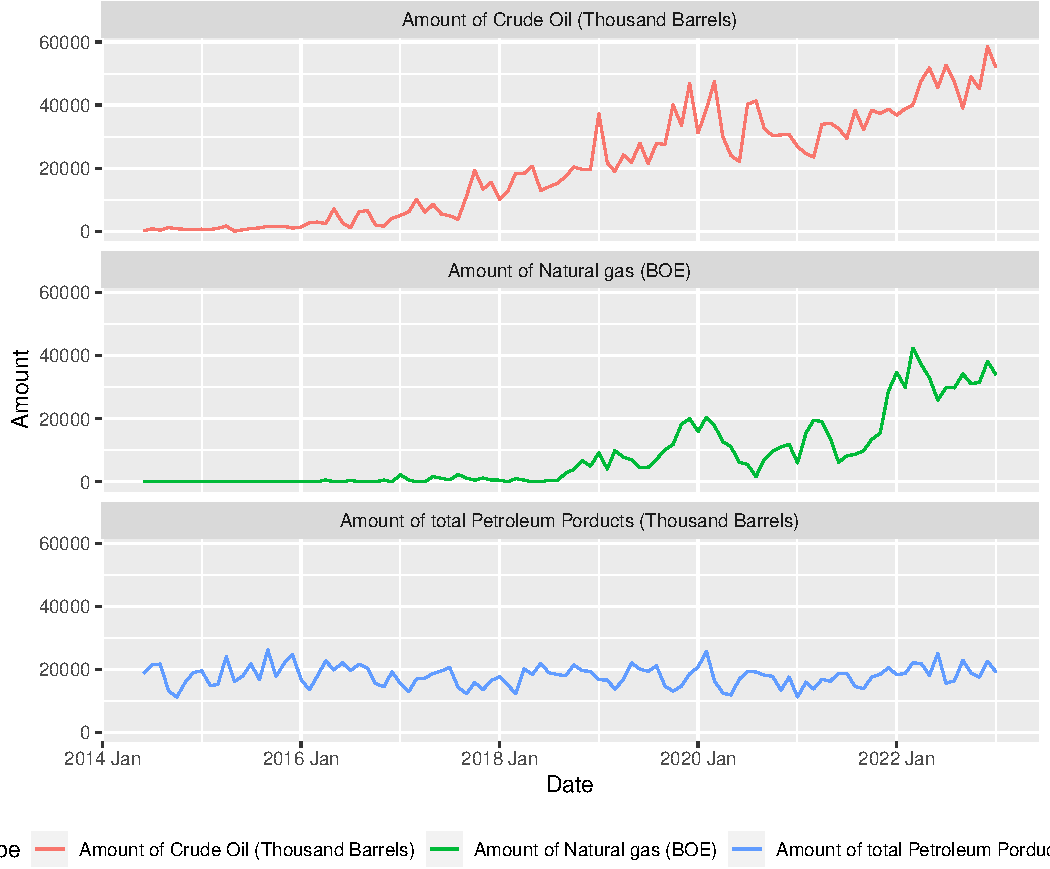
\includegraphics{draft1_files/figure-latex/overview by product-1.pdf}
\#\#\# 3. Time series decomposition \#\#\#\# 3.1. Adjustments

After a thorough review of the data, we determined that no adjustments
were necessary. We did not observe any calendar or population effects on
the monthly exports data, and the exports data is already presented in
barrels or barrels of oil equivalent (BOE), so no inflation adjustments
were required.

\hypertarget{transformations}{%
\paragraph{3.2. Transformations}\label{transformations}}

Given the nature of the three data sets that are being used: Crude Oil
Exports, Petroleum exports and Natural gas exports we decided that
certain transformations might be necessary for further analysis. Not
normal distribution of the data and differing variance were seen as
potential threat for correct conclusions. We identified Box-Cox
transformation as necessary to continue since it stabilizes the variance
of the data and makes the distribution more normal. This will improve
the reliability of the statistical tests and provide more accurate
results.

For Box-Cox transformation to be performed we found lambda for each time
series and than use it to transform the time series.

\hypertarget{decomposition}{%
\paragraph{3.3. Decomposition}\label{decomposition}}

\#\#\#STL Decomposition

\begin{verbatim}
## # A dable: 156 x 7 [1M]
## # Key:     .model [1]
## # :        Amount of Crude Oil (Thousand Barrels) = trend + season_year +
## #   remainder
##    .model     Date Amount of Crude Oil (Thousan~1  trend seaso~2 remai~3 seaso~4
##    <chr>     <mth>                          <dbl>  <dbl>   <dbl>   <dbl>   <dbl>
##  1 stl    2010 Feb                              0 -20.8    -31.4    52.2    31.4
##  2 stl    2010 Mar                              0 -18.7    222.   -203.   -222. 
##  3 stl    2010 Apr                              0 -16.6     41.9   -25.3   -41.9
##  4 stl    2010 May                              0 -14.4    383.   -369.   -383. 
##  5 stl    2010 Jun                              0 -13.1   -326.    339.    326. 
##  6 stl    2010 Jul                              0 -11.9   -435.    447.    435. 
##  7 stl    2010 Aug                              0 -10.6   -175.    186.    175. 
##  8 stl    2010 Sep                              0  -7.52   300.   -293.   -300. 
##  9 stl    2010 Oct                              0  -4.45   258.   -254.   -258. 
## 10 stl    2010 Nov                              0  -1.39  -196.    197.    196. 
## # ... with 146 more rows, and abbreviated variable names
## #   1: `Amount of Crude Oil (Thousand Barrels)`, 2: season_year, 3: remainder,
## #   4: season_adjust
\end{verbatim}

\begin{verbatim}
## # A dable: 156 x 7 [1M]
## # Key:     .model [1]
## # :        Amount of total Petroleum Porducts (Thousand Barrels) = trend +
## #   season_year + remainder
##    .model     Date Amount of total Petroleum Po~1  trend seaso~2 remai~3 seaso~4
##    <chr>     <mth>                          <dbl>  <dbl>   <dbl>   <dbl>   <dbl>
##  1 stl    2010 Feb                           5360  8579.  -4551.   1332.   9911.
##  2 stl    2010 Mar                           6323  9169.  -2557.   -290.   8880.
##  3 stl    2010 Apr                           8564  9759.    954.  -2150.   7610.
##  4 stl    2010 May                          10587 10349.   -116.    354.  10703.
##  5 stl    2010 Jun                          11776 10911.    618.    247.  11158.
##  6 stl    2010 Jul                          11143 11472.   1216.  -1544.   9927.
##  7 stl    2010 Aug                          12516 12033.   1104.   -621.  11412.
##  8 stl    2010 Sep                          13405 12570.   1109.   -274.  12296.
##  9 stl    2010 Oct                          16466 13107.    822.   2537.  15644.
## 10 stl    2010 Nov                          18301 13644.    567.   4090.  17734.
## # ... with 146 more rows, and abbreviated variable names
## #   1: `Amount of total Petroleum Porducts (Thousand Barrels)`, 2: season_year,
## #   3: remainder, 4: season_adjust
\end{verbatim}

\begin{verbatim}
## # A dable: 156 x 7 [1M]
## # Key:     .model [1]
## # :        Amount of Natural gas (BOE) = trend + season_year + remainder
##    .model     Date `Amount of Natural gas (BOE)` trend season~1 remain~2 seaso~3
##    <chr>     <mth>                         <dbl> <dbl>    <dbl>    <dbl>   <dbl>
##  1 stl    2010 Feb                             0 38.2    -39.0     0.829   39.0 
##  2 stl    2010 Mar                             0 33.2    -39.4     6.19    39.4 
##  3 stl    2010 Apr                             0 28.2    -20.1    -8.17    20.1 
##  4 stl    2010 May                             0 23.2    -16.4    -6.87    16.4 
##  5 stl    2010 Jun                             0 19.2    -59.8    40.7     59.8 
##  6 stl    2010 Jul                             0 15.1    -40.8    25.7     40.8 
##  7 stl    2010 Aug                             0 11.0     -6.19   -4.78     6.19
##  8 stl    2010 Sep                             0  7.98   -14.1     6.07    14.1 
##  9 stl    2010 Oct                             0  4.99   -29.0    24.0     29.0 
## 10 stl    2010 Nov                             0  2.01   108.   -110.    -108.  
## # ... with 146 more rows, and abbreviated variable names 1: season_year,
## #   2: remainder, 3: season_adjust
\end{verbatim}

\includegraphics{draft1_files/figure-latex/decomposition_plots-1.pdf}
\includegraphics{draft1_files/figure-latex/decomposition_plots-2.pdf}
\includegraphics{draft1_files/figure-latex/decomposition_plots-3.pdf}

We used STL decomposition to decompose the Box-Cox transformed time
series into three components: trend, seasonal, and residual. Four graphs
were plotted, three of which display the trend, seasonal, and residual
components, respectively while fourth one, the one at the top, represent
the export amounts from 2013 to 2023.

Looking at the graphs we see that in case of natural gas exports actual
patterns can only be seen appearing after approximately 2016 when the
U.S.

There are several conclusions to be drawn looking at the STL
decomposition. First of all, we can see clear trend in exports of crude
oil and natural gas while petroleum products does not have clear trend.
In both cases of exports of crude oil and natural gas we can clearly see
slight drops in exports after 2020 which can be explained by COVID 19
pandemic and continued growths after situation normalized. Another
observation worth mentioning is the fact that exports of two mentioned
products hits all time high around the year 2022. This can be explained
by huge declines of both products from Russia after sanction were
imposed.

Moreover, we can see seasonality in exports of all three products.That
is no surprise, given that all energy products are highly reactive to
different seasons.

After decomposing the data of all three time series and looking at each
components separately we decided that exports of petroleum products will
not be analysed further. Exports of petroleum products to OECD Europe
markets does not have clear trend therefore indicating that Russian
invasion in Ukraine did not have positive effect on growing imports from
US. This can be explained by the fact that embargo on refined oil
products from EU 27 was introduced as of 5 February 2023. Therefore,
Russian war on Ukraine and sanctions on Russia that followed did not
have any visible effect on US exports of petroleum products to OECD
Europe markets.

\hypertarget{the-forecasters-toolbox}{%
\subsection{4. The forecaster's toolbox}\label{the-forecasters-toolbox}}

\hypertarget{exploring-different-simple-forecasting-methods}{%
\paragraph{4.1. Exploring different simple forecasting
methods}\label{exploring-different-simple-forecasting-methods}}

\hypertarget{exponential-smoothing}{%
\subsection{5. Exponential smoothing}\label{exponential-smoothing}}

Yet to be started

\hypertarget{arima}{%
\subsection{6. ARIMA}\label{arima}}

Yet to be started

\hypertarget{other-forecasting-methods}{%
\subsection{7. Other forecasting
methods}\label{other-forecasting-methods}}

Yet to be started

\end{document}
